\section{Evaluation}
The evaluation section contains three distinct components: an analysis of the performance of a few popular methods, an overview of the Kaggle predictions, and a demonstration of the Nearest Neighbor Matchup Effects.
\subsection{Popular Methods}
March Madness prediction draws the attention of sport analysts and medias: notably, Nate Silver, Ken Pomeroy and the ESPN. In this section, we will score these three models according to Kaggle's loss function. Also since Nate Silver and Ken Pomeroy only published probabilities of each team advancing to a certain round, our first comparison is based on first round games (round of 64) only. 
  
We first notice that all three models concurred in win-loss predictions for all games  except one (Gonzaga vs OKST, 8 vs 9 in West). All three models have a similar pattern based on the predictions' deviation from 0.5. While most predictions suggest a easy win (prediction close to 1) or a close game (prediction close to 0.5), predictions around 0.75 are relatively rare. This is may because the first around game are relatively easy prediction.

Silver's predictions also adapted a more aggressive style than the other two. His predictions, on average, have the highest 0.2818  deviation from 50-50 prediction, Pomeroy averages the lowest, 0.2388. But this difference seems to be independent of the result through, for the first around, Pomeroy has the best score of 0.4632, Silver scored 0.4664 and 0.4709 for ESPN. 

We have also examined the luck factor with popular models. After flipping the results of five overtime games, we noticed a completely reverse of the rankings of scores with the ESPN model ranks first (0.4631) and Pomeroy ranks third (0.5027), Silver remains second (0.5025).

The scores look competitive but they are based on the easiest prediction in the tournament. To obtain a fuller comparison, we compute team-to-team prediction based marginal advancement probabilities and  the overall scores are ESPN (0.5795), Silver(0.5988) and Pomeroy (0.6278). The overall scores are substantially lower than the first round's which is a common observation for most Kaggle entries.    

To sum up, popular models exhibit similarities in many aspect which can be useful for future Kaggle competitors. But result-wise, none have shown advantages over the majority of Kaggle entries. 

\subsection{Kaggle Leaderboard}
\andyc{is this section appropriate here?  Consider the flow of the once paper the pieces come together}
\subsection{Nearest Neighbor Matchup Effects}
To demonstrate the efficacy of our method, we first fit Equation~\ref{eq:RS} using a well known rating system, the Sagarin ratings. After fitting this model, $\rho$ is calibrated based on historical results from the previous seven years NCAA tournaments. Note seven years was chosen as this is the complete history of the team level characteristics used to find neighbors of teams. The log loss for 2014 for the entire range of $\rho$ can be seen in Figure~\ref{fig:result} and the value that was selected based on historical calibration of $\rho =0.2$.
\begin{figure}[h!]
\centering
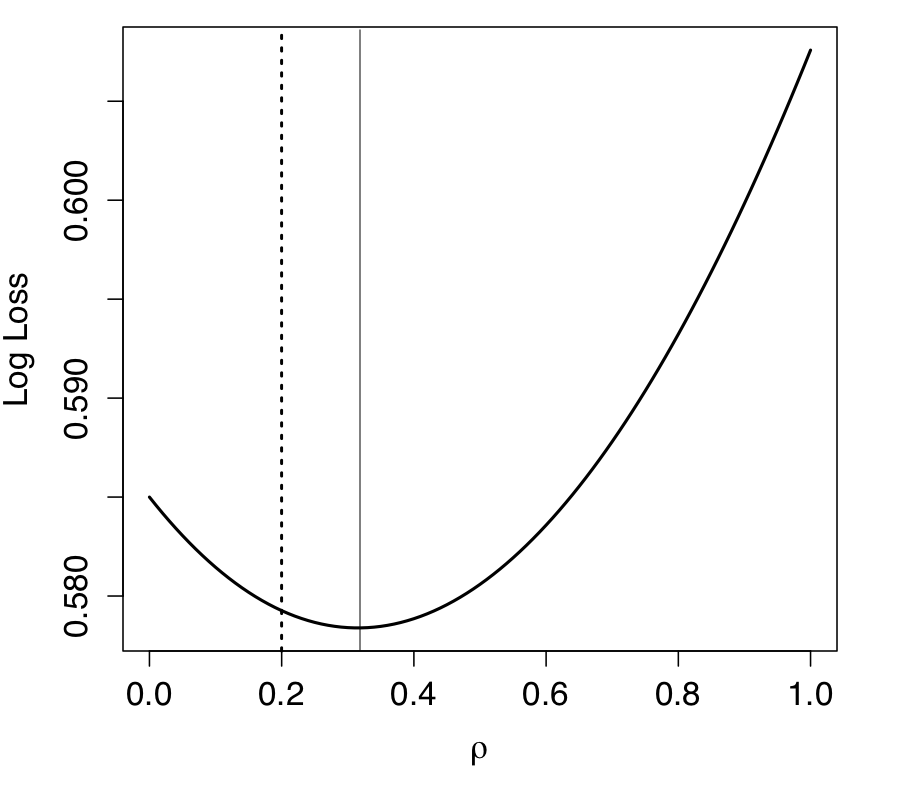
\includegraphics[width=.7\textwidth]{results_2014.pdf}
\caption{Log loss for no matchup effect = red, log loss for optimized $\rho$ = blue}
\label{fig:result}
\end{figure} 
The selected $\rho$ value results in a reduction in loss. A modest improvement is also seen in classification error from (0.365 to 0.350) although this is only a single game difference. The matchup effect, particularly with smaller $\rho$ values, will have a lesser effect on classification error than that of the loss functions like the log loss. This is because it will only shift the expected point differential a fairly small margin, so the only games in which classification error would change are those that are nearly dead heat games to begin with.

To illustrate the matchup effects, consider Table~\ref{tab:change} which contains the ten games that saw the largest shift in expected point differential. This table contains expected point differentials (team1 - team2) denoted as Point Diff for the relative strength model (RS) as well as the matchup effects (ME).  Similarly probabilities of team 1 winning and realized loss for each model are depicted.  Finally the actual point differential is shown.
\begin{table}[h!]
\caption{ Ten games with largest point differential change when implementing Nearest Neighbor Matchup Effects model versus a relative strength model}
\scriptsize
\centering
\begin{tabular}{|cc | ccc | ccc | c|c|}
  \hline
  \hline
 team 1 & team 2 & Point Diff:RS & Prob:RS & Loss:RS & Point Diff:ME & Prob:ME & Loss:ME & Point Diff\\ 
  \hline
 Cal Poly & Wichita St & -18.69 & 0.04 & 0.04 & -17.10 & 0.06 & 0.06 &  -27\\ 
 UConn & St. Joes &4.29 & 0.65 & 0.43 & 6.18 & 0.71 & 0.34 & 8\\ 
 Dayton & Stanford & -2.16 & 0.42 & 0.86 & 0.94 & 0.53 & 0.63 & 10 \\ 
 Dayton & Syracuse & -6.34 & 0.28 & 1.27 & -4.05 & 0.36 & 1.03 & 2\\ 
 Kentucky & Michigan & -3.71 & 0.37 & 1.00 & -2.08 & 0.42 & 0.86 &  3\\ 
 UMass & Tennessee &-3.05 & 0.39 & 0.49 & -4.83 & 0.33 & 0.40 & -19\\ 
 Memphis & Virginia & -6.34 & 0.28 & 0.33 & -8.91 & 0.21 & 0.23 & -18\\ 
 Michigan & Tennessee & 5.37 & 0.69 & 0.37 & 3.49 & 0.62 & 0.47 & 2\\ 
 Michigan & Texas & 8.05 & 0.77 & 0.26 & 5.85 & 0.70 & 0.35 & 14\\ 
 Syracuse & W. Mich. & 12.65 & 0.88 & 0.13 & 15.01 & 0.92 & 0.09 & 24\\ 
   \hline
   \hline
\end{tabular}
\label{tab:change}
\end{table}
The key takeaway from this table is the loss for the predictions under each methodology. On this particular subset of games, the matchup effects model performs considerably better than the typical model under the log loss (.446 to .520). As the other games see minimal matchup effects, the results are essentially the same.  Specifically from the table, Dayton, in particular had a series of games against Syracuse and Stanford that were more favorable than a relative strength model using Sagarin would suggest.